\documentclass[a4paper]{article}
\usepackage[utf8]{ctex}
\usepackage{amsfonts}
\usepackage{amsthm}
\usepackage{graphicx}

\title{\textbf{作业四:二叉树和节点的逻辑设计}}
\author{李沁霞 \\ 统计学 3210300363}
\date{\today}

\begin{document}

\maketitle

\section{设计思路}
节点是数据结构上不可少的元素。它可以用于描述二叉树的顶点和级别。由于节点的有效功能,使得每次构造新的模板就需要创建节点。我们可以构造一个Node模板使它继承与新的模板上。这样就方便多了!

二叉树是一种非线性数据结构,其中可以有0、1或2个节点构成的树。每个节点有左指针,右指针和数据元素组成。二叉树主要用于插入、遍历和删除数据的树。二叉树使用的遍历函数有inorderT()、postorderT()和preorderT()。

二叉搜索树是具有结构化节点组织的二叉树。二叉搜索树是用于排序、检素和搜索数据的树。它具有特殊的搜索功能,可以在树上找到最大值(findMax())和最小值(findMin())。其中最常见的二叉搜索树的类型有AVL树。

AVL树是一种自平衡的二叉搜索树。AVL树主要是解决树上不平衡的高度。它继承二叉搜索树的所有函数,其中添加的函数有rotate()、balance()和height()。

\begin{center}
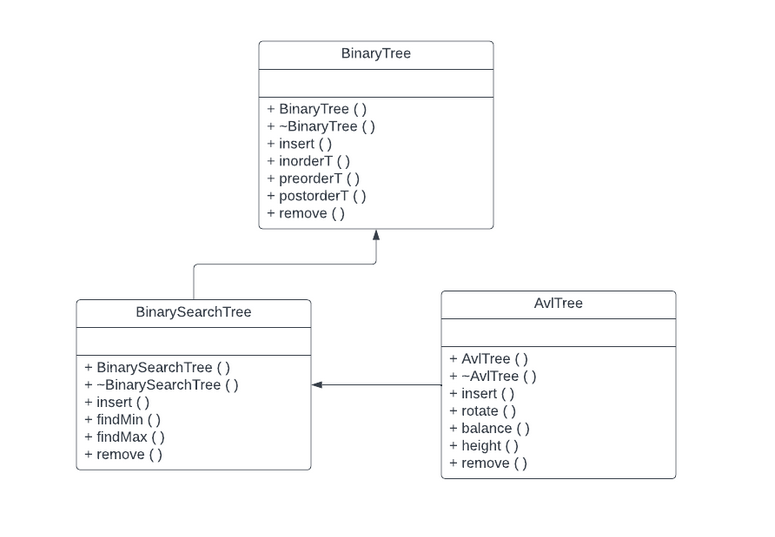
\includegraphics[scale=0.5]{uml}
\end{center}

\end{document}
